\section{Expérience en biologie (7 points)}

La courbe expérimentale de la figure ci-dessous donne, en fonction du temps $t$ en minutes, la consommation $C(t)$ d'oxygène d'une personne à l'instant $t$, en millilitres par minutes.

\begin{center}
	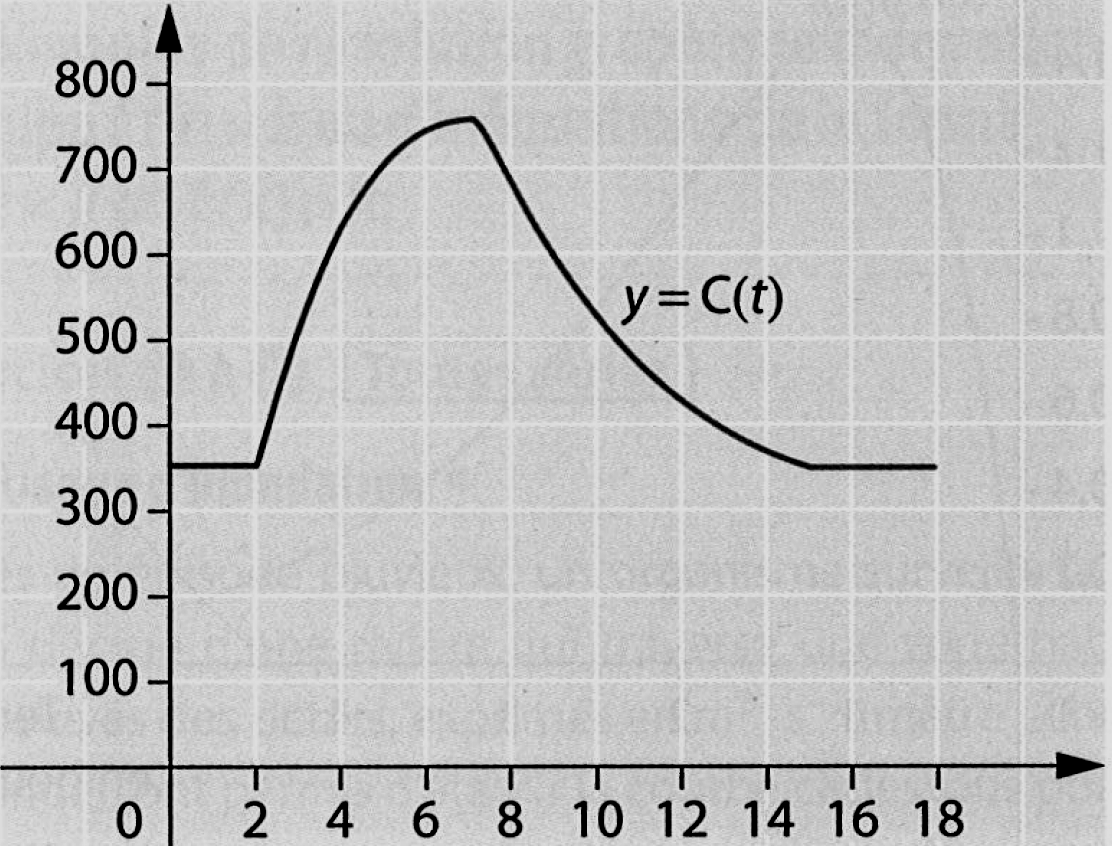
\includegraphics[scale=0.4]{img/bio}	
\end{center}

Avant le début des mesures, la personne étudiée se trouvait dans un bain à $\num{36.5} $°C où elle reste pendant les deux premières minutes d'observation, avant d'être placée pendant 5 minutes dans un bain à 30 °C, puis remise dans un bain à $\num{36.5} $ °C jusqu'à la fin de l'étude.

\begin{questions}
	\question[2] Déterminer graphiquement les consommations en oxygène aux instants $t=4$, $t=6$, $t=10$ et $t=12$, c'est à dire $C(4)$, $C(6)$, $C(10)$ et $C(12)$.
	
	\question[2] \`A quels instants la consommation en oxygène est-elle égale à :
	\begin{parts}
		\part 500;
		\part 700;
		\part 800;
		\part 350.
	\end{parts}

	\question[1] Entre quelles valeurs varie la consommation d'oxygène lorsque $t$ varie entre 0 et 18 ?
	
	\question [2] Dresser le tableau de variation de la fonction $C$ définie sur $\left[   0;18\right] $
	%\begin{parts}
		%\part[1] Déterminer graphiquement les coordonnées du sommet de la courbe.
	%	\part
	%\end{parts}
\end{questions}